Any information gets deteriorated or lost over time.

\begin{enumerate}
\item Paintings gets deteriorated over time and has to be renovated.
\item Some of the words spoken by teacher in the class is missed due to noise.
\end{enumerate}

To be able to over come this issue , i.e to be able to detect and correct errors during transmission of information in digital system "coding theory" is developed.
In digital system, information are transmitted as strings of \(0\) and \(1\). The idea of coding theory is to append some extra digits to the information and use this to detect and possibly correct the errors during transmission.
So the fundamental of the coding theory in computer system is the manipulation of strings of binary digits. The proper and complete manipulation of these strings is possibly only if the space of the strings is a field. This field is finite so this field is a \textbf{Galois field}. This is where the application of Galois theory comes.
Another advantage of using field is that the space of code forms a vector space over the base field. \\
The widely used field for coding in electronically transmitting device is the field \({\mathbb{Z}}_2\) which is the field \(GF(2)\) consisting of \(0\) and \(1\). Recent works has shown that it is possible to extend codes to more general type of numbers called rings. This rings are called "Galois rings".\\

The non-empty set of symbols for the code \(\mathcal{A}\) called \textbf{alphabet}. A finite sequence of elements from \(\mathcal{A}\) is called a \textbf{word} over \(\mathcal{A}\). Let \(\mathcal{A}^*\) be the set of all words over \(\mathcal{A}\). A subset \(C\) of \(\mathcal{A}\) is called a code.
If the cardinality of the alphabet \(\mathcal{A}\) is \(q\) then the code \(C\) is called \(q-ary code\). For \(q=2\) it is called binary and for \(q=3\) it is caled terniary.

\section{Linear Codes}
Let \(K=GF(q)\) be a Galois field. Then a finite extension of \(K\) of dimension \(n\) is \(V=GF(q)^n=GF(q^n)\).
\begin{definition}
  A linear code \(C\) is a subspace of \(V\). \\
  The code \(C\) has dimension \(k \leq n\) and the length \(n\). It is called a \((n,k)\) code.
\end{definition}

The usefulness of linear code is that they are vector spaces over the base field so they have a basis. All the code words can be generated with this basis. Instead of storing all \(2^k\) number of code words (for \(k\)-dimensional binary codes), storing only \(k\) basis elements is sufficient which saves massive storage.\\[2mm]
Let \(C\) be \((n,k)\) code which is a subspace of \(V\).

\begin{definition}[Generator Matrix]
  Let \(\{v_1, v_2,...,v_k\}\) be a basis of \(C\). A generator matrix is the \(k \times n\)
  \[G=\begin{pmatrix}
      v_1\\
      v_2\\
      .\\
      .\\
      .\\
      v_k
    \end{pmatrix}
  \]
\end{definition}
\vspace{2mm}

\begin{definition}[Parity check matrix]
  The dual code of \(C\) is the set \(C^{\perp}=\{x \in V \;| \; x.y=0 \;\; \forall y \in V \}\). The dual code is a code in itself and has dimension \(n-k\).\\
  The \(C^{\perp}\) is linear so it has a generator matrix. A generator matrix \(H\) of \(C^{\perp}\) is called a parity check matrix.
\end{definition}

\begin{theorem}
  If \(G=(I_{k \times k},A_{k \times (n-k)})\) is a generator matrix of an \((n,k)\) code \(C\) then its parity check matrix is \(H=(I_{(n-k) \times (n-k)}, A'\) where \(A'\) is the transpose of \(A\).
\end{theorem}

\begin{definition}
  The \textit{Hamming distance} between \(v,w \in V\) is defined by \(d_h(v,w)=|\{i\;|\; v_i \neq w_i;\; 1 \leq i \leq n \}|\).\\
  The \textit{minimum distance} of a code \(C\) is defined as \(min\{d_h(v,w)\;|\; d_h(v,w) \neq 0, v,w \in C\}\).\\
  The weight of a vector is its distance from zero and the \textit{minimum weight} of a code \(C\) is the minimum weight of all non-zero weights of the vectors in \(C\).
\end{definition}

\begin{theorem}
  A linear code \(C\) with minimum weight \(d\) can correct strings having number of errors up to \(t= \lfloor (d-1)/2 \rfloor\).
\end{theorem}

\section{Illustration}
To apply \((n,k)\) coding first we need to group our information into blocks of length \(k\).
\(u_1,...,u_k\),  \(u_k,...,u_{2k}\),... . This space has dimension \(k\). Now these block of codes are encoded separately each to a code of length \(n\) as shown.

\vspace{5mm}
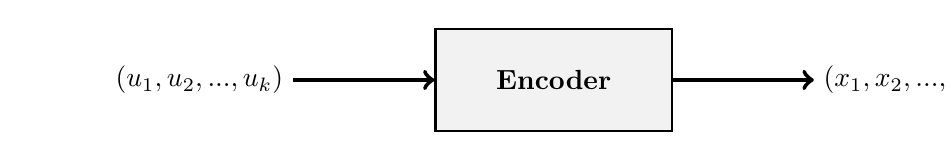
\begin{tikzpicture}
  \hspace{1cm}
  \node [] (u) {\((u_1,u_2,...,u_k\))};
  \node[
  right of=u,
  rectangle,
  draw,
  thick,
  fill=gray!10,
  minimum width=30mm,
  minimum height=13mm,
  xshift=35mm] (e) {\bfseries Encoder};

  \node[right of=e, xshift=35mm] (x) {\((x_1,x_2,...,x_n)\)};

  \draw[->,ultra thick] (u)--(e);
  \draw[->,ultra thick] (e)--(x);
\end{tikzpicture}

\vspace{4mm}
\noindent
Mathematically, the encoded vector \(x\) is obtained form the original vector \(u\) using the generator matrix \(G\) by the relation \(x=uG\).\\[5mm] To continue and complete the diagram.\\

\vspace{4mm}
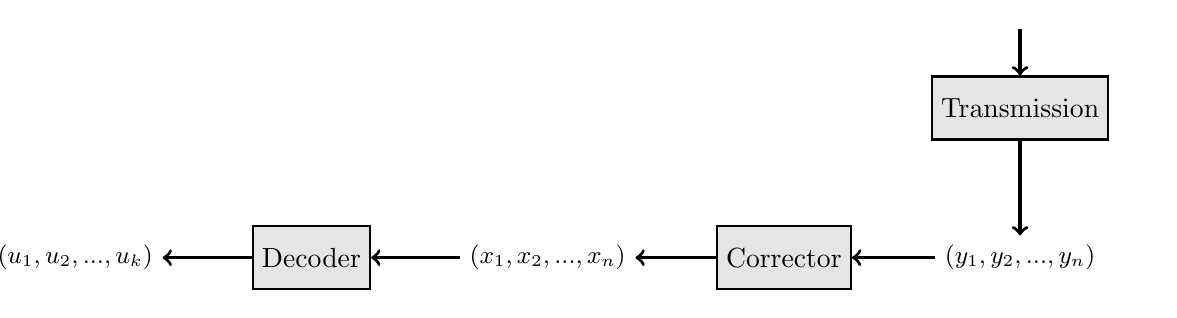
\begin{tikzpicture}
  \hspace{-5mm}
  \node[
  rectangle,
  draw,
  thick,
  fill=gray!20,
  minimum width=13mm,
  minimum height=8mm,
  ] (t) {Transmission};

  \node[below of=t, yshift=-9mm] (y) {\small \((y_1,y_2,...,y_n\))};

  \node[
  left of=y,
  rectangle,
  draw,
  thick,
  fill=gray!20,
  minimum width=13mm,
  minimum height=8mm,
  xshift=-20mm] (c) {Corrector};

  \node[left of=c, xshift=-20mm] (x) {\small \((x_1,x_2,...,x_n)\)};

  \node[
  left of=x,
  rectangle,
  draw,
  thick,
  fill=gray!20,
  minimum width=13mm,
  minimum height=8mm,
  xshift=-20mm] (d) {Decoder};

  \node[left of=d, xshift=-20mm] (u) {\small \((u_1,u_2,...,u_k\))};


  \draw[->,very thick] (0,1)--(t);
  \draw[->,very thick] (t)--(y);
  \draw[->,very thick] (y)--(c);
  \draw[->,very thick] (c)--(x);
  \draw[->,very thick] (x)--(d);
  \draw[->,very thick] (d)--(u);
\end{tikzpicture}

\vspace{9mm}
\section{Syndrome Decoding}
\begin{definition}
  The syndrome of a vector \(y \in V\) is defined as \\ \(syn(y)=\begin{pmatrix}
    y.h_1\\
    y.h_2\\
    .\\
    .\\
    .\\
    y.h_{n-k}
  \end{pmatrix}\), \hspace{12mm} where \(\begin{pmatrix}
    h_1 \\ h_2\\ .\\ .\\ .\\ h_{n-k}
  \end{pmatrix}\) is the parity check matrix of \(C\).
\end{definition}
\vspace{3mm}
Now the code \(C\) is a subgroup of \(V\) under addition. Moreover, it is a normal subgroup of \(V\).
\begin{theorem}
  Two vectors in \(V\) have the same syndrome if and only if they are in the same co-set of \(C\).
\end{theorem}
\clearpage

\subsection{Decoding Process}
Suppose the signal received is the vector \(y\).
\begin{enumerate}
\item First we determine its syndrome, \(syn(y)\).
\item Determine the co-set of \(C\) containing \(syn(y)\), say \(e + C\).
\item Then \(y=e+x\) for some \(x \in C\). This implies \(x=y-e\). Since \(x \in C\), this \(x\) is the required decoding of \(y\).
\end{enumerate}
This \(e\) is also called "error vector".
\vspace{2mm}

\begin{example}
  Consider a generator matrix \(G=\begin{pmatrix}
    1 & 0 & 1 & 0\\
    0 & 1 & 1 & 1
  \end{pmatrix}\). Then the parity check matrix is \(H=\begin{pmatrix}
    1 & 1 & 1 & 0\\
    0 & 1 & 0 & 1
  \end{pmatrix}\). And the code generated by \(G\) is  \(C=\{(0,0,0,0),(1,0,1,0),(0,1,1,1),(1,0,1,1)\} \;\; \subset GF(2)^{4}\).\\

  Suppose the received vector is \(y=(1,1,1,0)\). Then \(y \not \in C\) so the information is distorted from the original information. To get the original information:\\
  \(syn(y)= \begin{pmatrix}
    y.h_1 \\ y.h_2
  \end{pmatrix} = \begin{pmatrix}
    1 \\ 1
  \end{pmatrix}\) where \(h_1\) is the first row and \(h_2\) is the second row of \(H\).\\
  Now if \(e=(0,1,0,0)\) then \(e+C=\begin{pmatrix}
    1 \\ 1
  \end{pmatrix}\) so \(y-e=(1,1,1,0)-(0,1,0,0)=(1,0,1,0) \in C\) is the original information.

\end{example}


\section{Perfect Code}
The code \(C \subseteq V\) as of above is perfect if the union of all the spheres of radius \(t\) about its code-words is the vector space \(V\).\\
This code is \(C\) is called perfect because every received vector with the number of errors given by \(t\) can be decoded to a code-word of \(C\).

\begin{example}
  The code \(C=V\) is a perfect code. This code cannot correct any errors because every possible code word is in the \(C\). Therefore this perfect code is trivial.
\end{example}

\begin{example}
  The general binary Hamming code \(H_r\), \(r \in \mathbb{N}\) whose parity check matrix \(H\) column consisting of non-zero r-tuples.
\end{example}

\section{Cyclic Code}
The code \(C\) as of above is cyclic if \((a_0,a_1,...,a_{n-1}) \in C \implies (a_{n-1},a_0,...,a_{n-2}) \in C\).\\

Suppose \(C\) is a code over a Galois field \(F=GF(q)\). Then there exist a correspondence \(\Phi : C \mapsto F[x]/(x^n-1)\) such that \((a_0,a_1,...,a_{n-1})\longmapsto a_0+a_1x+a_2x^2+...+a_{n-1}x^{n-1}\).\\
This shows that the cyclic code \(C\) can be embedded into the ring \(R_n=F[x]/(x^n-1)\).

\begin{theorem}
  \begin{enumerate}
  \item A subset \(S\) of \(R_n\) corresponds to a cyclic code if and only if \(S\) is an ideal of \(R_n\) and
  \item if \(S=(g(x))\) if and only if  \(g(x)\) divides \(x^n-1\)
  \end{enumerate}
\end{theorem}

This theorem determines all cyclic codes. They are ideals of \(R_n\) and these ideals are generated by the polynomials that divides \(x^n-1\).

\begin{example}
  The divisors of \(x^3-1 \in F=GF(2)^{3}\) are \(1, x+1, x^2+x+1, x^3-1\).\\
  For \(g(x)=x+1\) we have \(F[x]/(g(x))=\{(0),(1+x),(1+x^2),(x+x^2)\}\) so the corresponding cyclic code is \(\{(0,0,0),(1,1,0),(1,0,1),(0,1,1)\}\).
\end{example}

\vspace{5mm}
Similar to general linear codes which are defined using the generator matrix or the parity-check matrix, cyclic codes are defined using generator polynomial or parity-check polynomial and due to this efficient algebraic decoding algorithm exist.

\subsection{Usages}
\begin{enumerate}
\item The \((3,1)\) binary code is used in the short-range wireless communication system like \(Bluetooth^{TM}\).
  \item The Hamming Code \((7,4)\) is used in memory devices like RAM.
\end{enumerate}
